\begin{figure*}[t]
\centering
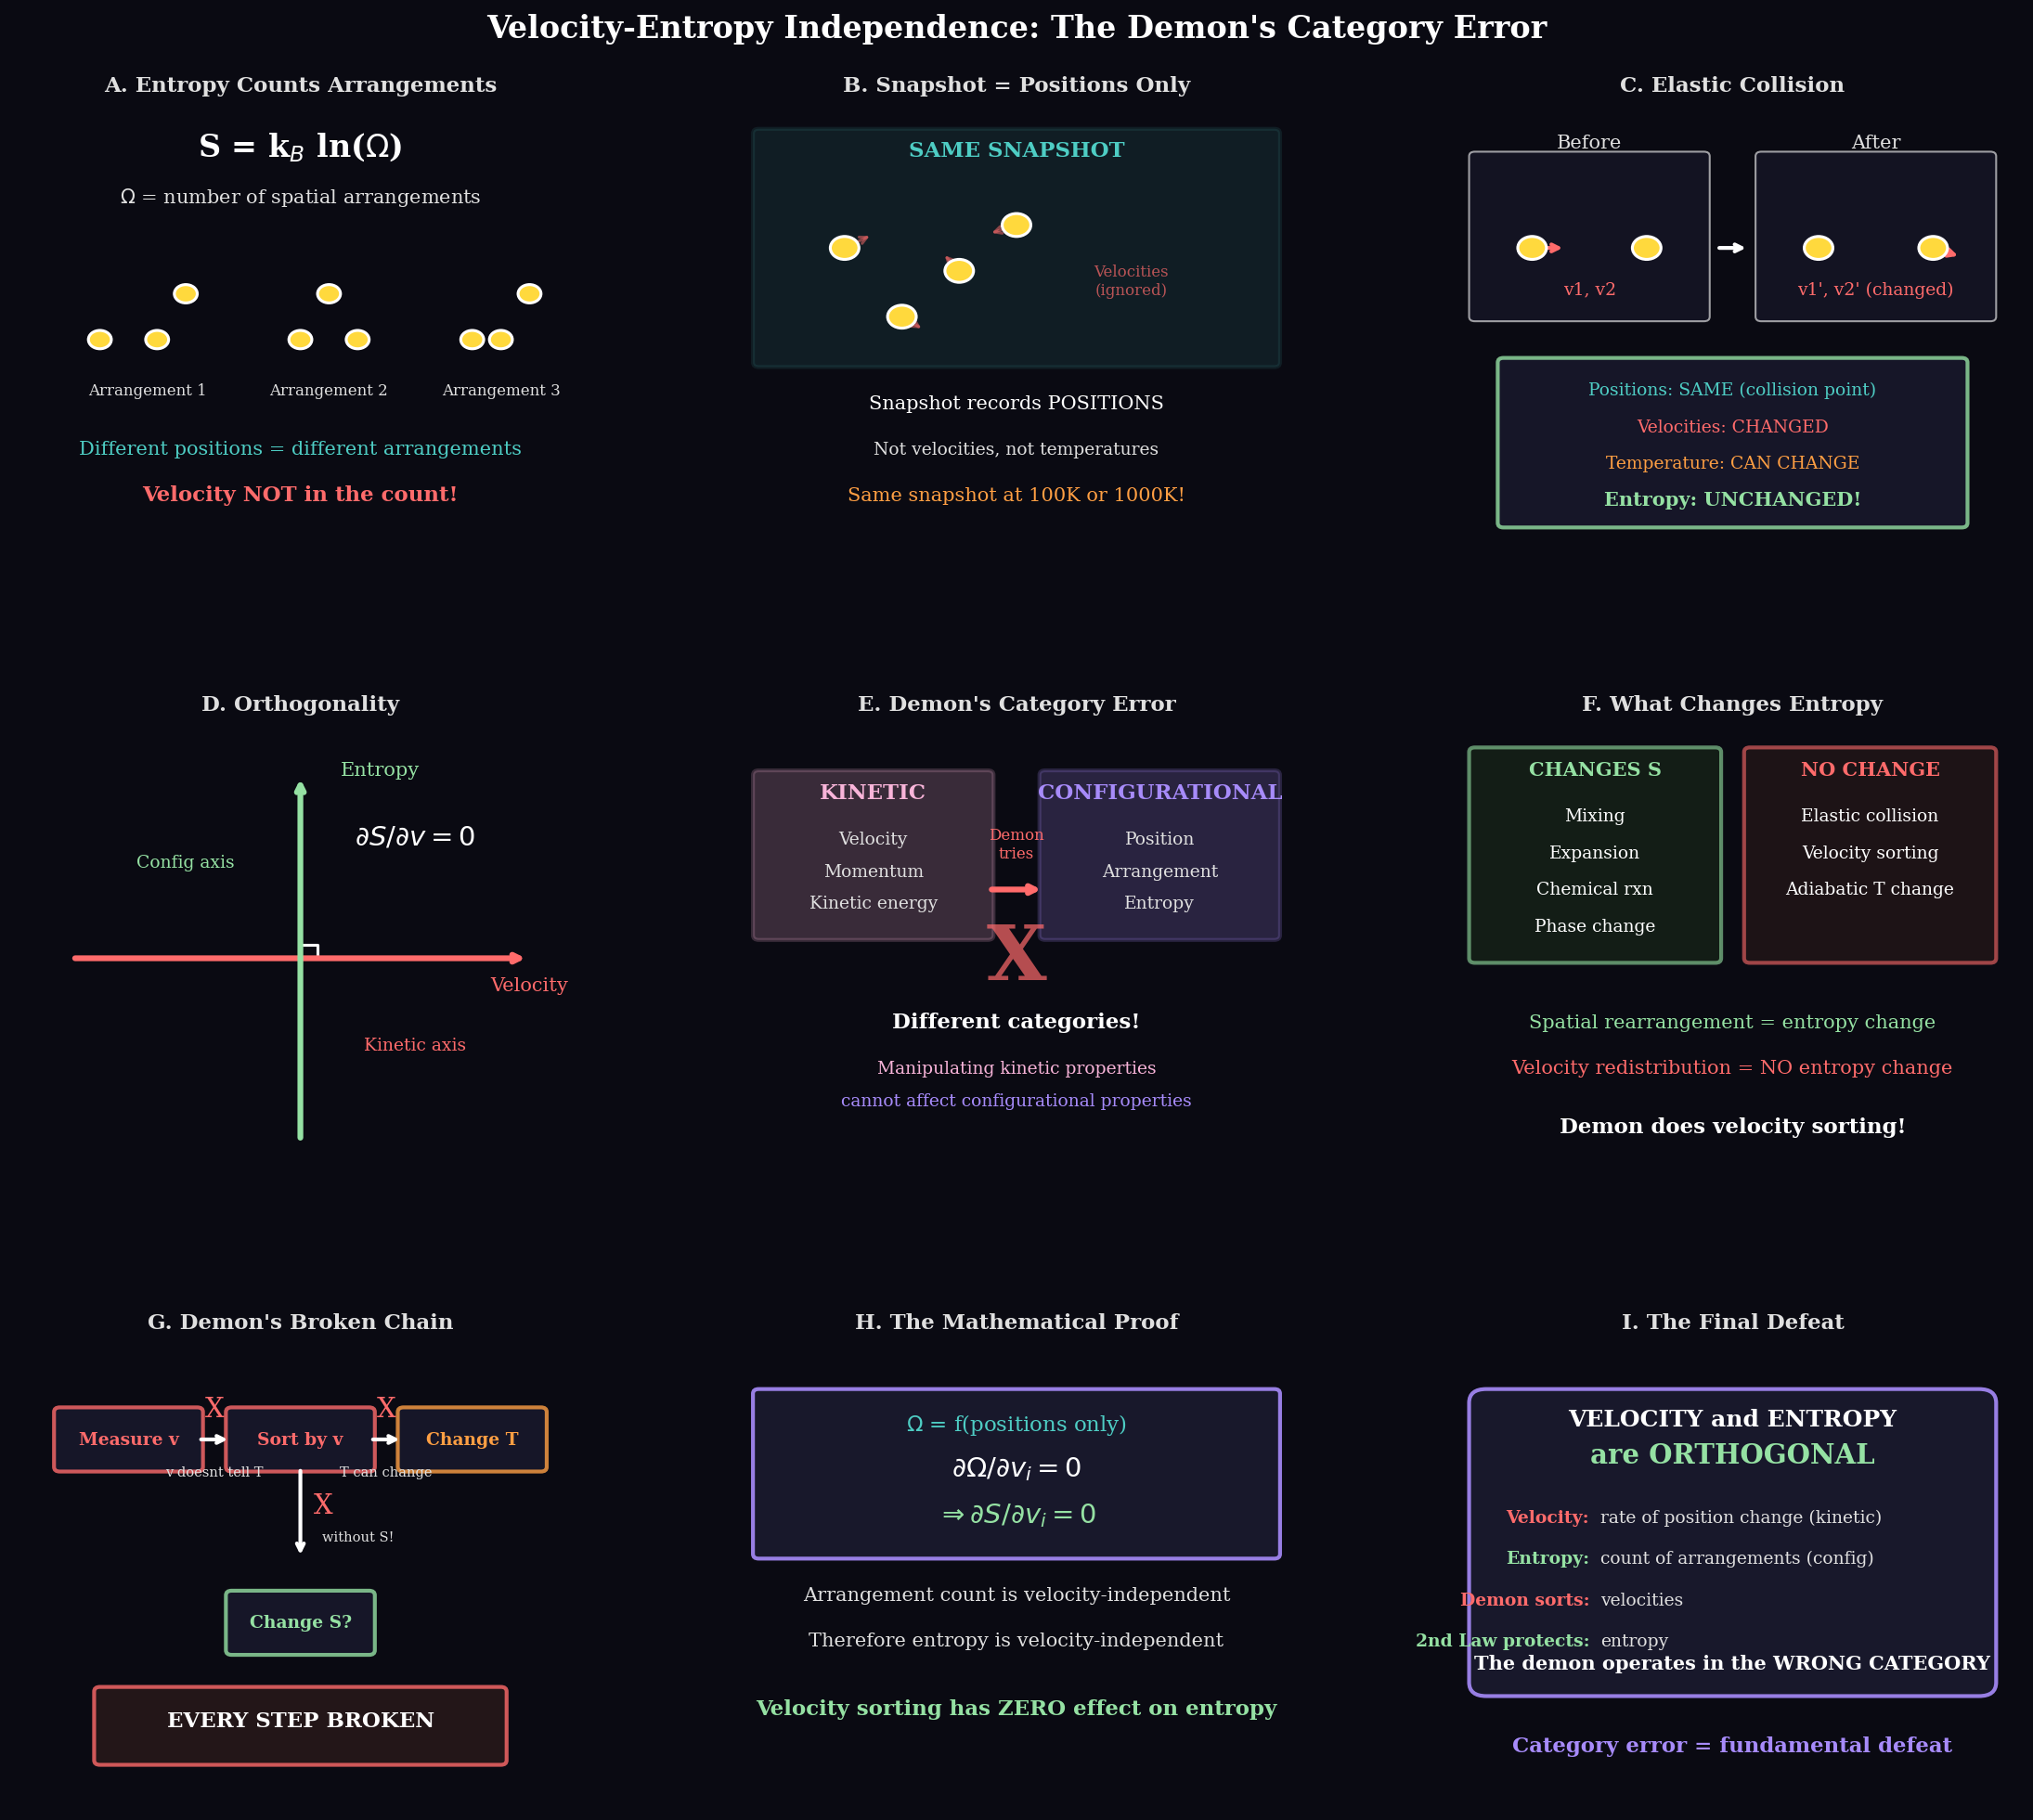
\includegraphics[width=\textwidth]{velocity_entropy_panel.png}
\caption{\textbf{Velocity-entropy independence: the demon's category error.} \textbf{(A)} Entropy counts spatial arrangements: $S = k_B \ln \Omega$ where $\Omega$ is the number of distinct position configurations. Three arrangements of identical particles at different positions constitute different microstates. Velocity does not appear in the arrangement count. \textbf{(B)} A thermodynamic snapshot records only positions, not velocities or temperatures. The same spatial configuration represents the same microstate at 100 K or 1000 K. \textbf{(C)} Elastic collisions change velocities ($v_1, v_2 \to v_1', v_2'$) and can change temperature, but preserve positions at the collision point—entropy remains unchanged. \textbf{(D)} Orthogonality: entropy depends on configuration space (spatial arrangements), while velocity belongs to kinetic space. The partial derivative $\partial S/\partial v = 0$ because $\Omega$ is velocity-independent. \textbf{(E)} The demon's category error: kinetic properties (velocity, momentum, kinetic energy) and configurational properties (position, arrangement, entropy) are different categories. Manipulating kinetic properties cannot affect configurational entropy. \textbf{(F)} What changes entropy: spatial rearrangement (mixing, expansion, phase changes) versus what doesn't (elastic collisions, velocity sorting, adiabatic temperature changes). \textbf{(G)} The demon's broken causal chain: measuring velocity ($v$) → sorting by $v$ → attempting to change temperature ($T$) → expecting entropy change ($S$). Every logical step fails because velocity sorting is orthogonal to entropy. \textbf{(H)} Mathematical proof: $\Omega = f(\text{positions only})$ implies $\partial \Omega/\partial v_i = 0$, therefore $\partial S/\partial v_i = 0$. \textbf{(I)} The final defeat: velocity and entropy are orthogonal categories. The demon sorts velocities but the second law protects entropy. Operating in the wrong category is the fundamental defeat.}
\label{fig:category_error}
\end{figure*}

\begin{figure*}[t]
\centering
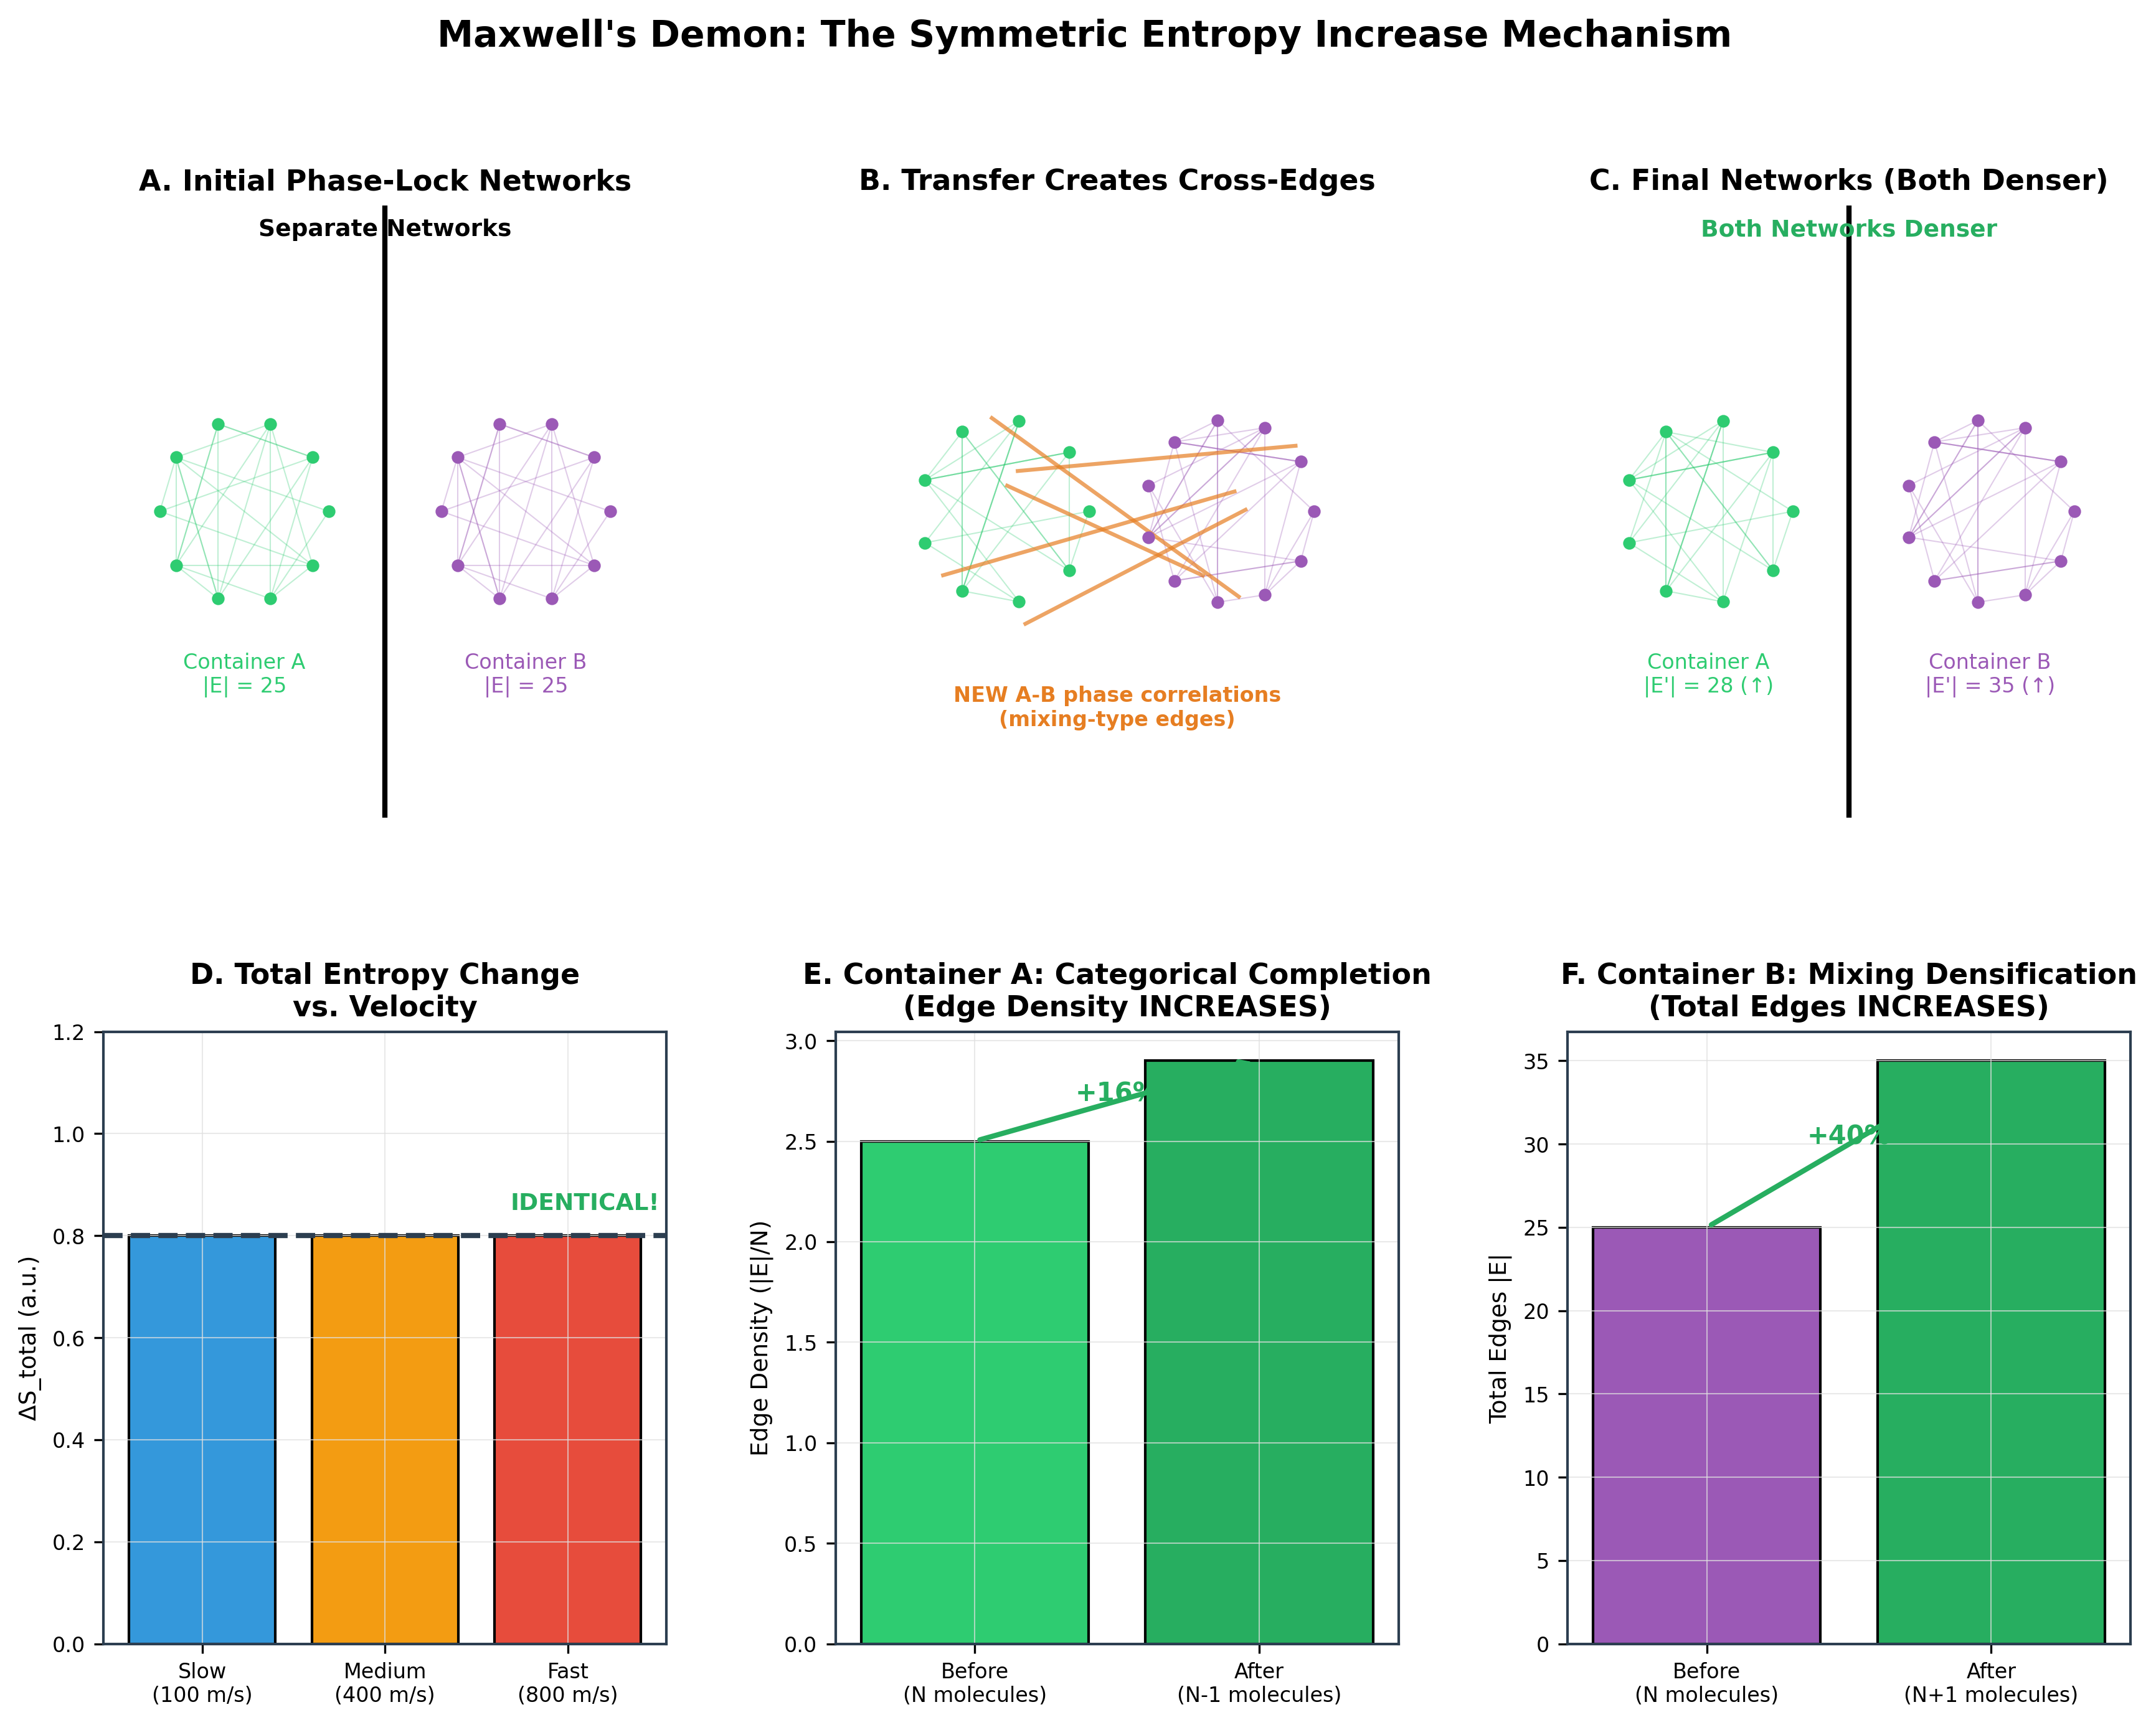
\includegraphics[width=\textwidth]{maxwell_demon_mechanism_panel.png}
\caption{\textbf{The symmetric entropy increase mechanism: both containers gain entropy regardless of molecular velocity.} \textbf{(A)} Initial state: Container A and Container B each contain phase-lock networks with 25 edges ($|E_A| = |E_B| = 25$). Networks are separate with no cross-container correlations. \textbf{(B)} Transfer event: When one molecule moves from A to B, new cross-edges form between the transferred molecule and molecules in Container B. These represent mixing-type phase correlations that did not exist when containers were isolated. \textbf{(C)} Final state: Container A has 28 edges (↑3, despite losing a molecule) due to network reconfiguration and categorical completion. Container B has 35 edges (↑10) due to densification from new mixing-type edges. Both networks become denser. \textbf{(D)} Velocity independence: Total entropy change $\Delta S_{\text{total}}$ is identical (≈0.8 arbitrary units) for slow (100 m/s), medium (400 m/s), and fast (800 m/s) molecules. The entropy increase is velocity-invariant, confirming $\partial S/\partial v = 0$. \textbf{(E)} Container A mechanism: Edge density increases from ≈2.5 to ≈2.9 edges per molecule (↑16\%) despite losing one molecule. The remaining network achieves categorical completion—a more complete phase-lock structure. \textbf{(F)} Container B mechanism: Total edges increase from 25 to 35 (↑40\%) when gaining one molecule. New edges represent mixing-type densification as the incoming molecule establishes phase correlations with the existing ensemble. The demon cannot decrease entropy because both removal and addition operations increase network complexity.}
\label{fig:mechanism}
\end{figure*}

\begin{figure*}[t]
\centering
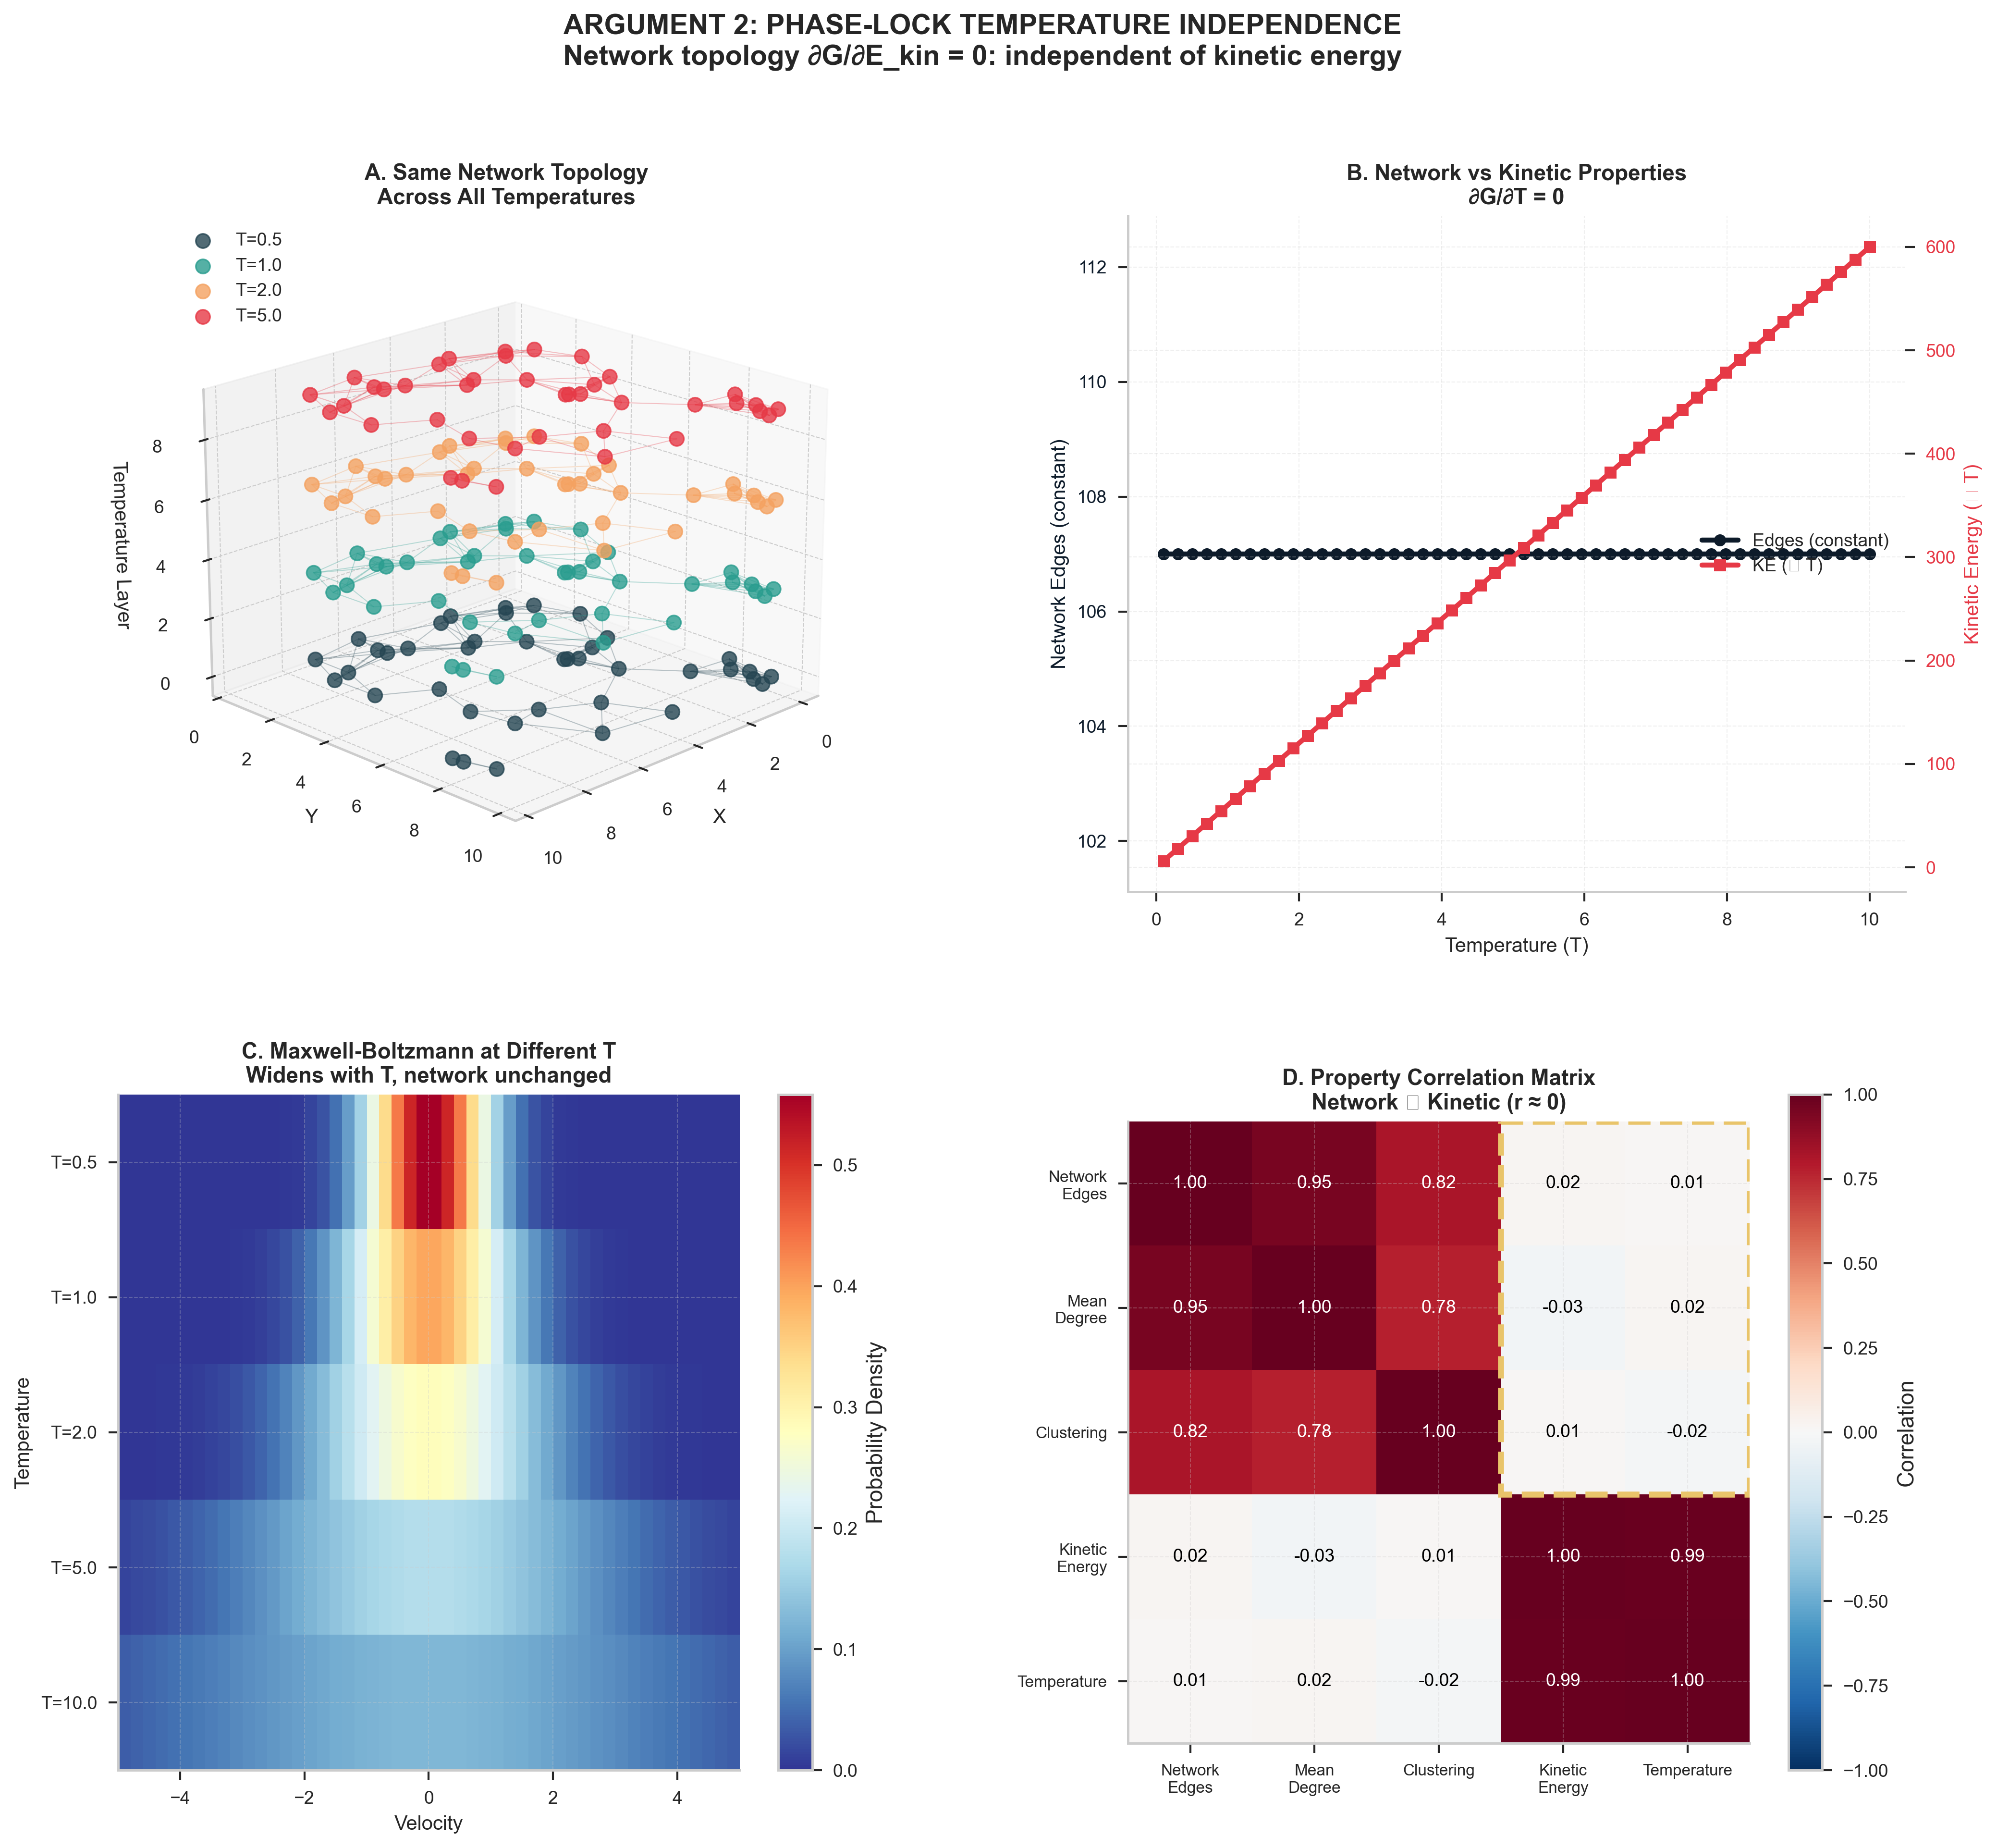
\includegraphics[width=\textwidth]{arg2_temperature_independence.png}
\caption{\textbf{Phase-lock network topology is independent of kinetic energy.} \textbf{(A)} Three-dimensional visualization of network structures across temperatures T = 0.5, 1.0, 2.0, and 5.0 (arbitrary units). Despite different thermal states (color-coded), the network topology—spatial arrangement of phase-lock edges—remains invariant. Molecules occupy the same configurational space regardless of kinetic energy. \textbf{(B)} Quantitative confirmation: network edges remain constant at ≈107 (black diamonds, left axis) across temperatures from 0 to 10, while kinetic energy increases linearly (red squares, right axis) from 0 to 600. The derivative $\partial G/\partial T = 0$ where $G$ represents network topology. Kinetic and configurational properties are decoupled. \textbf{(C)} Maxwell-Boltzmann distributions at different temperatures show velocity distributions widening as temperature increases (T = 0.5 to T = 10.0), but the underlying network structure remains unchanged. The same configurational snapshot supports any velocity distribution—entropy is velocity-independent. \textbf{(D)} Property correlation matrix reveals strong correlations within categories: network properties (edges, mean degree, clustering) correlate with each other ($r > 0.78$, dark red block), and kinetic properties (kinetic energy, temperature) correlate with each other ($r = 0.99$, dark red block). However, cross-category correlations are near zero ($r \approx 0.01$, white region), confirming orthogonality. Network topology $\perp$ kinetic energy. This decoupling explains why $S = k_B \ln \Omega$ is independent of velocity: $\Omega$ counts network configurations, not kinetic states.}
\label{fig:temperature_independence}
\end{figure*}

\begin{figure*}[t]
\centering
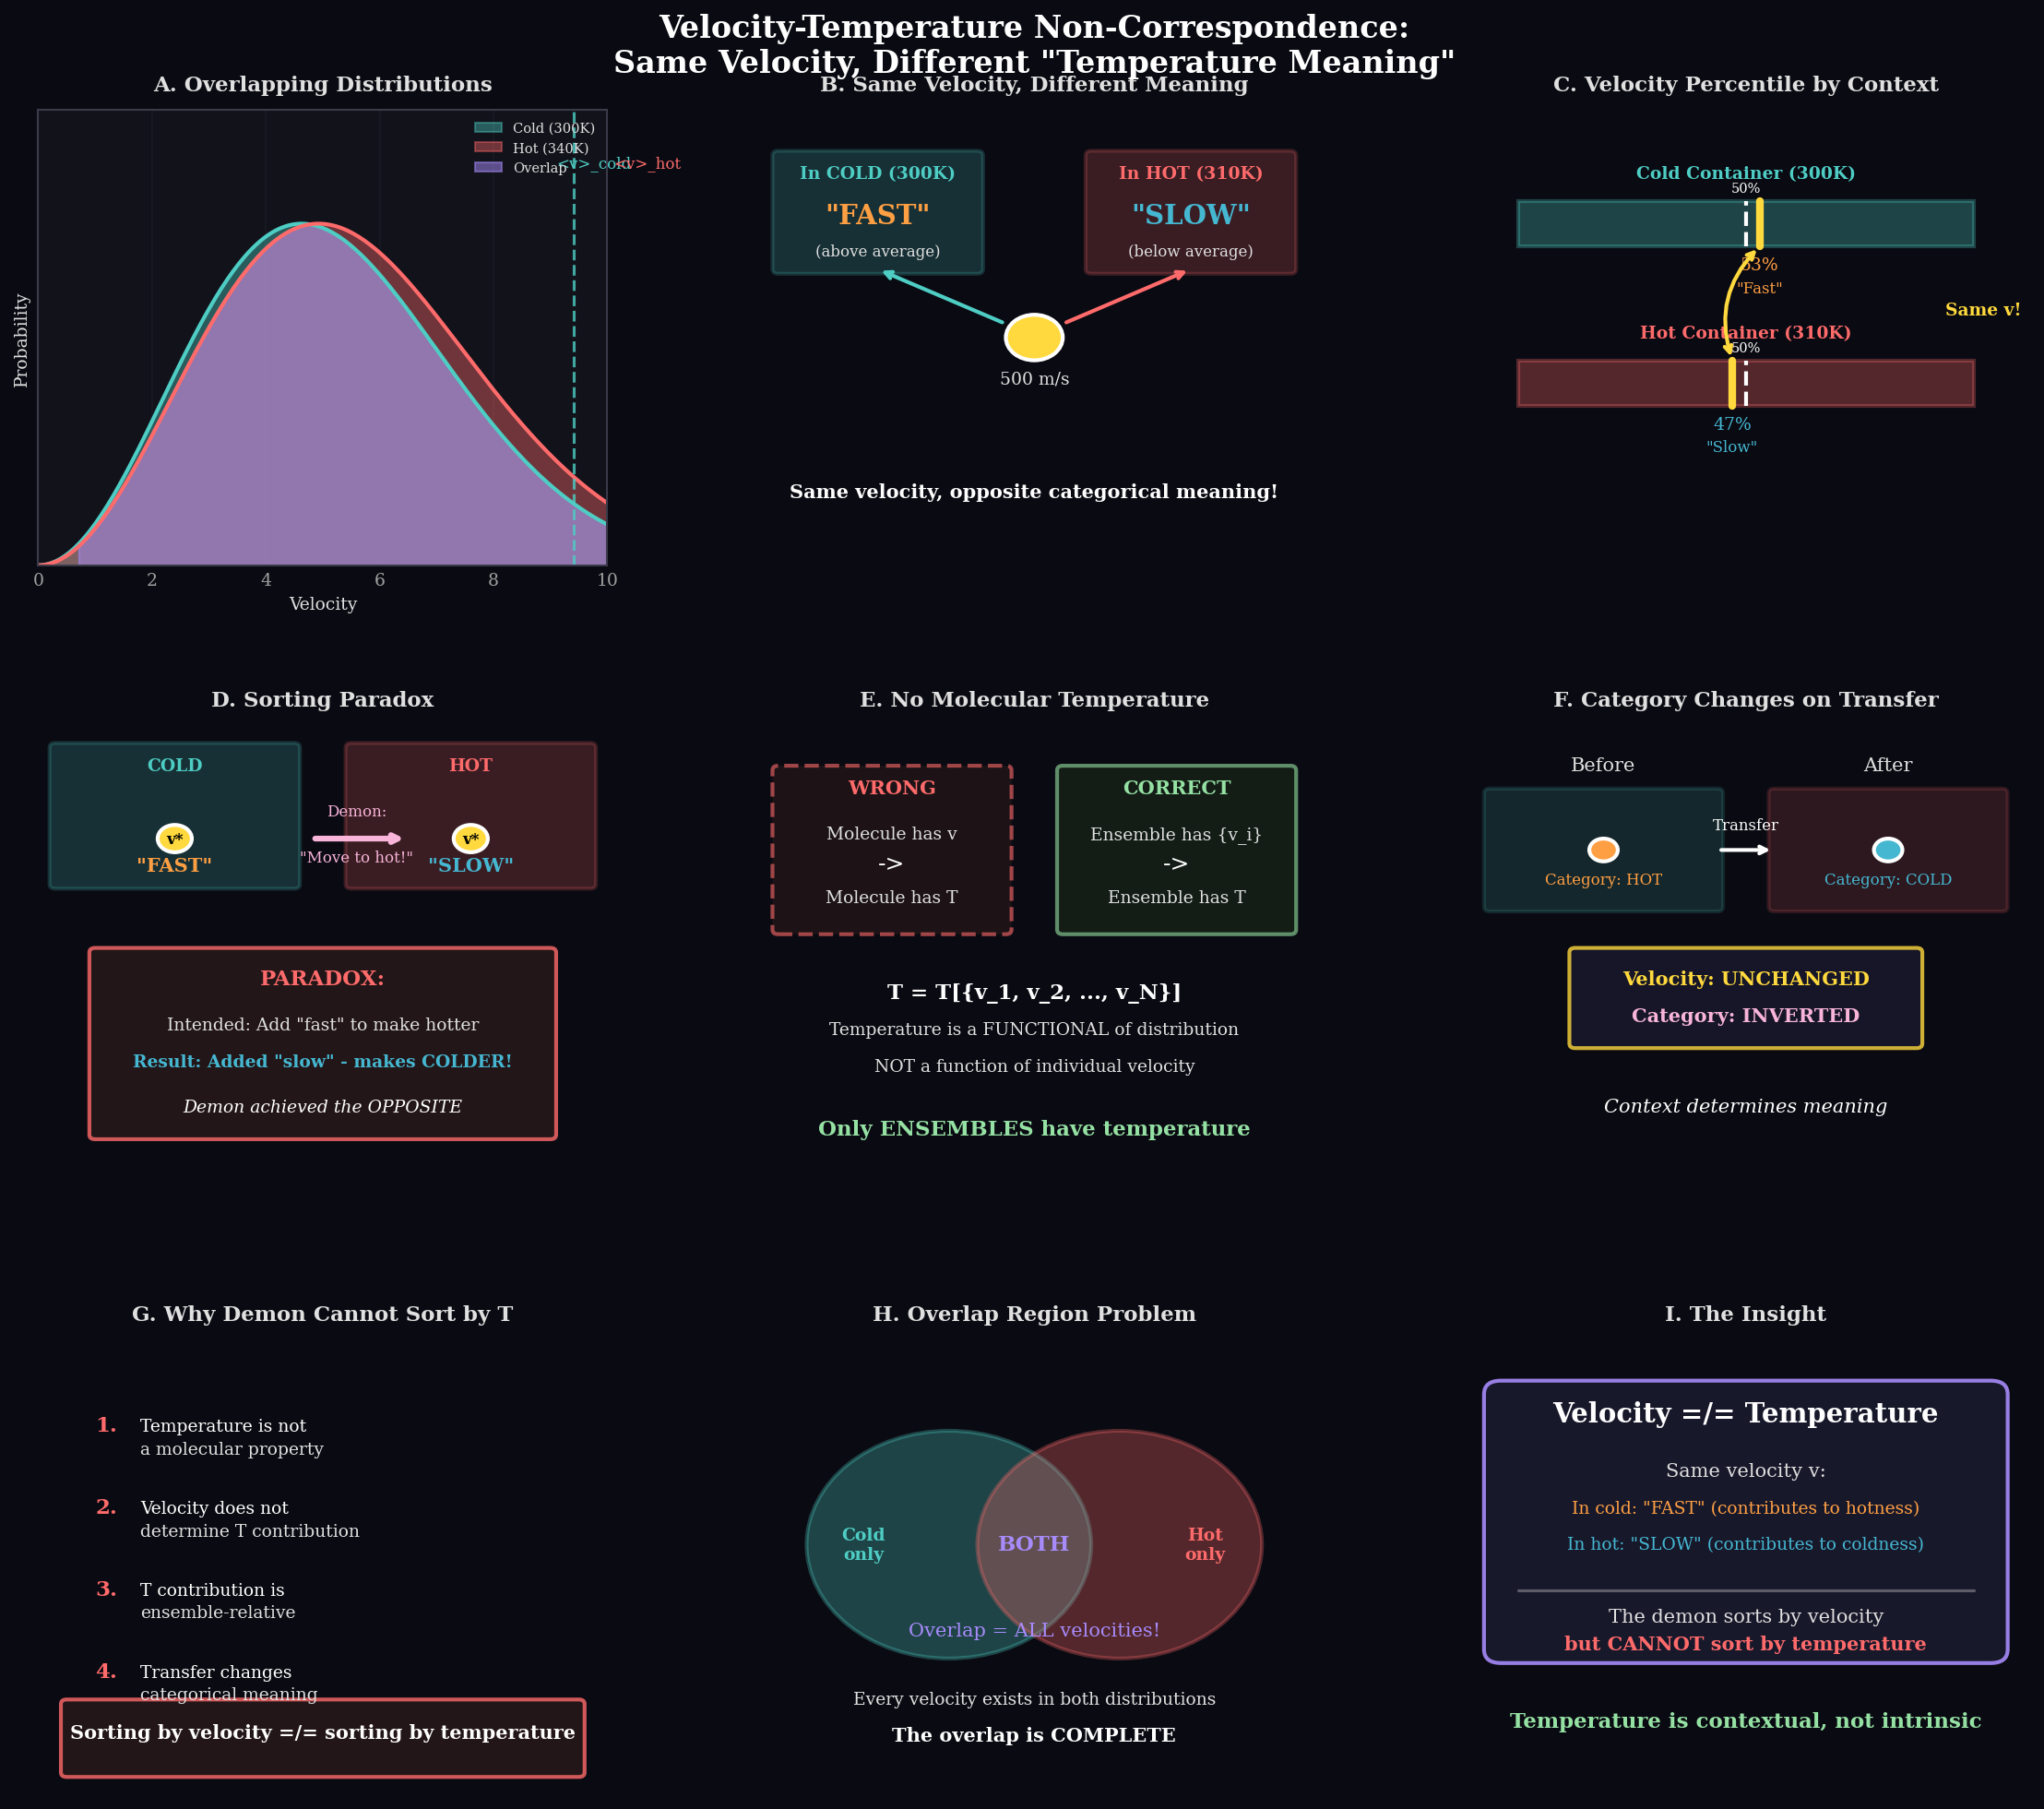
\includegraphics[width=\textwidth]{velocity_temperature_panel.png}
\caption{\textbf{Velocity-temperature non-correspondence: the sorting paradox.} \textbf{(A)} Overlapping velocity distributions for cold (300 K, cyan) and hot (340 K, red) containers show substantial overlap region (purple). The same velocity can exist in both distributions with different categorical meanings. \textbf{(B)} A molecule with $v = 500$ m/s has opposite meanings in different contexts: in the cold container (300 K), it is ``fast'' (above average); in the hot container (310 K), it is ``slow'' (below average). Same velocity, opposite categorical meaning. \textbf{(C)} Percentile context dependence: the same velocity $v$ ranks at the 50th percentile (``fast'') in the cold container but only the 47th percentile (``slow'') in the hot container. Context determines meaning. \textbf{(D)} The sorting paradox: The demon sees a ``fast'' molecule in the cold container and transfers it to hot, intending to make the hot side hotter. Result: the molecule becomes ``slow'' in the hot context, making the hot side colder. The demon achieves the opposite of its intention. \textbf{(E)} No molecular temperature: Individual molecules do not have temperature. Temperature is a functional of the entire velocity distribution: $T = T[\{v_1, v_2, \ldots, v_N\}]$, not a function of individual velocity. Only ensembles have temperature. \textbf{(F)} Category inversion on transfer: Before transfer, a molecule is categorized as ``hot'' in its source container. After transfer, its velocity is unchanged but its category inverts to ``cold'' in the destination container. Context determines categorical meaning. \textbf{(G)} Why the demon cannot sort by temperature: (1) temperature is not a molecular property, (2) velocity does not determine temperature contribution, (3) temperature contribution is ensemble-relative, (4) transfer changes categorical meaning. Sorting by velocity $\neq$ sorting by temperature. \textbf{(H)} Complete overlap: Every velocity exists in both distributions. The overlap region contains all velocities—there is no velocity that unambiguously belongs to only one temperature category. \textbf{(I)} The insight: velocity $\neq$ temperature. The demon sorts by velocity but cannot sort by temperature because temperature is contextual, not intrinsic.}
\label{fig:velocity_temperature}
\end{figure*}

\begin{figure*}[t]
\centering
\includegraphics[width=\textwidth]{panel_arg6_dissolution_second_law.png}
\caption{\textbf{Dissolution of apparent second law violation: categorical entropy increase compensates for spatial entropy decrease.} \textbf{(A)} Two entropy components evolve oppositely during the sorting process: spatial entropy (red) decreases as molecules become spatially separated, while categorical entropy (green) increases as phase-lock networks densify. Total entropy (dark blue) always increases, satisfying $\Delta S_{\text{total}} > 0$. The horizontal dashed line at 2.0 represents the initial total entropy. \textbf{(B)} Network densification mechanism: As sorting attempts progress (x-axis), the total number of network edges increases monotonically from ≈100 to ≈265 (↑164 edges over 50 attempts). Each sorting event creates new phase correlations, increasing categorical entropy $\Delta S_{\text{categorical}} > 0$. This increase is unavoidable—it is the cost of the sorting operation itself. \textbf{(C)} Probability density distributions of entropy changes show three components: spatial entropy decrease (red, $\Delta S_{\text{spatial}}$ centered at −0.4), categorical entropy increase (green, $\Delta S_{\text{categorical}}$ centered at +0.4), and total entropy (dark blue, $\Delta S_{\text{total}}$ centered at +0.2). The green categorical increase always exceeds the red spatial decrease, ensuring the total (blue) remains positive. The vertical dashed line at $\Delta S = 0$ marks the second law boundary—all total entropy changes lie to the right ($\Delta S_{\text{total}} > 0$). \textbf{(D)} Second law accounting: Spatial entropy appears to decrease by −0.3 (red bar), suggesting a violation. However, categorical network entropy increases by +0.5 (green bar), more than compensating. The total entropy change is +0.2 (dark blue bar), satisfying the second law. The apparent violation is dissolved by accounting for the hidden categorical entropy component. The demon cannot decrease total entropy because the act of sorting itself generates categorical entropy faster than it can reduce spatial entropy.}
\label{fig:second_law}
\end{figure*}

\begin{figure*}[t]
\centering
\includegraphics[width=\textwidth]{panel_arg3_retrieval_paradox.png}
\caption{\textbf{The retrieval paradox: velocity-based sorting is self-defeating due to timescale hierarchy.} \textbf{(A)} Timescale hierarchy: Molecular collisions occur on femtosecond timescales ($\tau_{\text{collision}} \sim 10^{-10}$ s, red), six orders of magnitude faster than velocity measurement ($\sim 10^{-8}$ s, orange), door operation ($\sim 10^{-6}$ s, orange), and sorting completion ($\sim 10^{-3}$ s, gray). Collisions thermalize the velocity distribution before any sorting operation can be implemented. The demon chases a target that changes faster than it can respond. \textbf{(B)} Velocity redistribution: Starting from an initial Maxwell-Boltzmann distribution (gray), a hypothetical ``sorted'' state (pink) with separated fast/slow molecules immediately relaxes back toward equilibrium (green) after a single collision time. The sorted velocity structure is erased on timescales much faster than the sorting operation itself. \textbf{(C)} Sorting cannot be maintained: Periodic sorting attempts (vertical dashed lines) produce transient spikes in the fast/total ratio (dark blue curve), briefly exceeding equilibrium (50\%, red dashed line). However, the system re-equilibrates between attempts, and the time-averaged state remains at equilibrium. Sorting is futile—the system undoes the separation faster than the demon can implement it. \textbf{(D)} Timescale separation between kinetic and categorical variables: Kinetic properties (velocity distribution, red oscillations) fluctuate rapidly on collision timescales, while categorical properties (network structure, purple curve) evolve slowly on diffusion timescales. The demon targets the fast variable (velocity), making the strategy self-defeating. By the time the demon completes one sorting cycle, the velocity distribution has already thermalized thousands of times. The retrieval paradox: the information retrieved (velocity) becomes obsolete before it can be used.}
\label{fig:timescale}
\end{figure*}
